\teaser{
	\centering
	\vspace{-1.75cm}
	\addtolength{\tabcolsep}{-4.5pt}
	\newlength{\insetLen}
	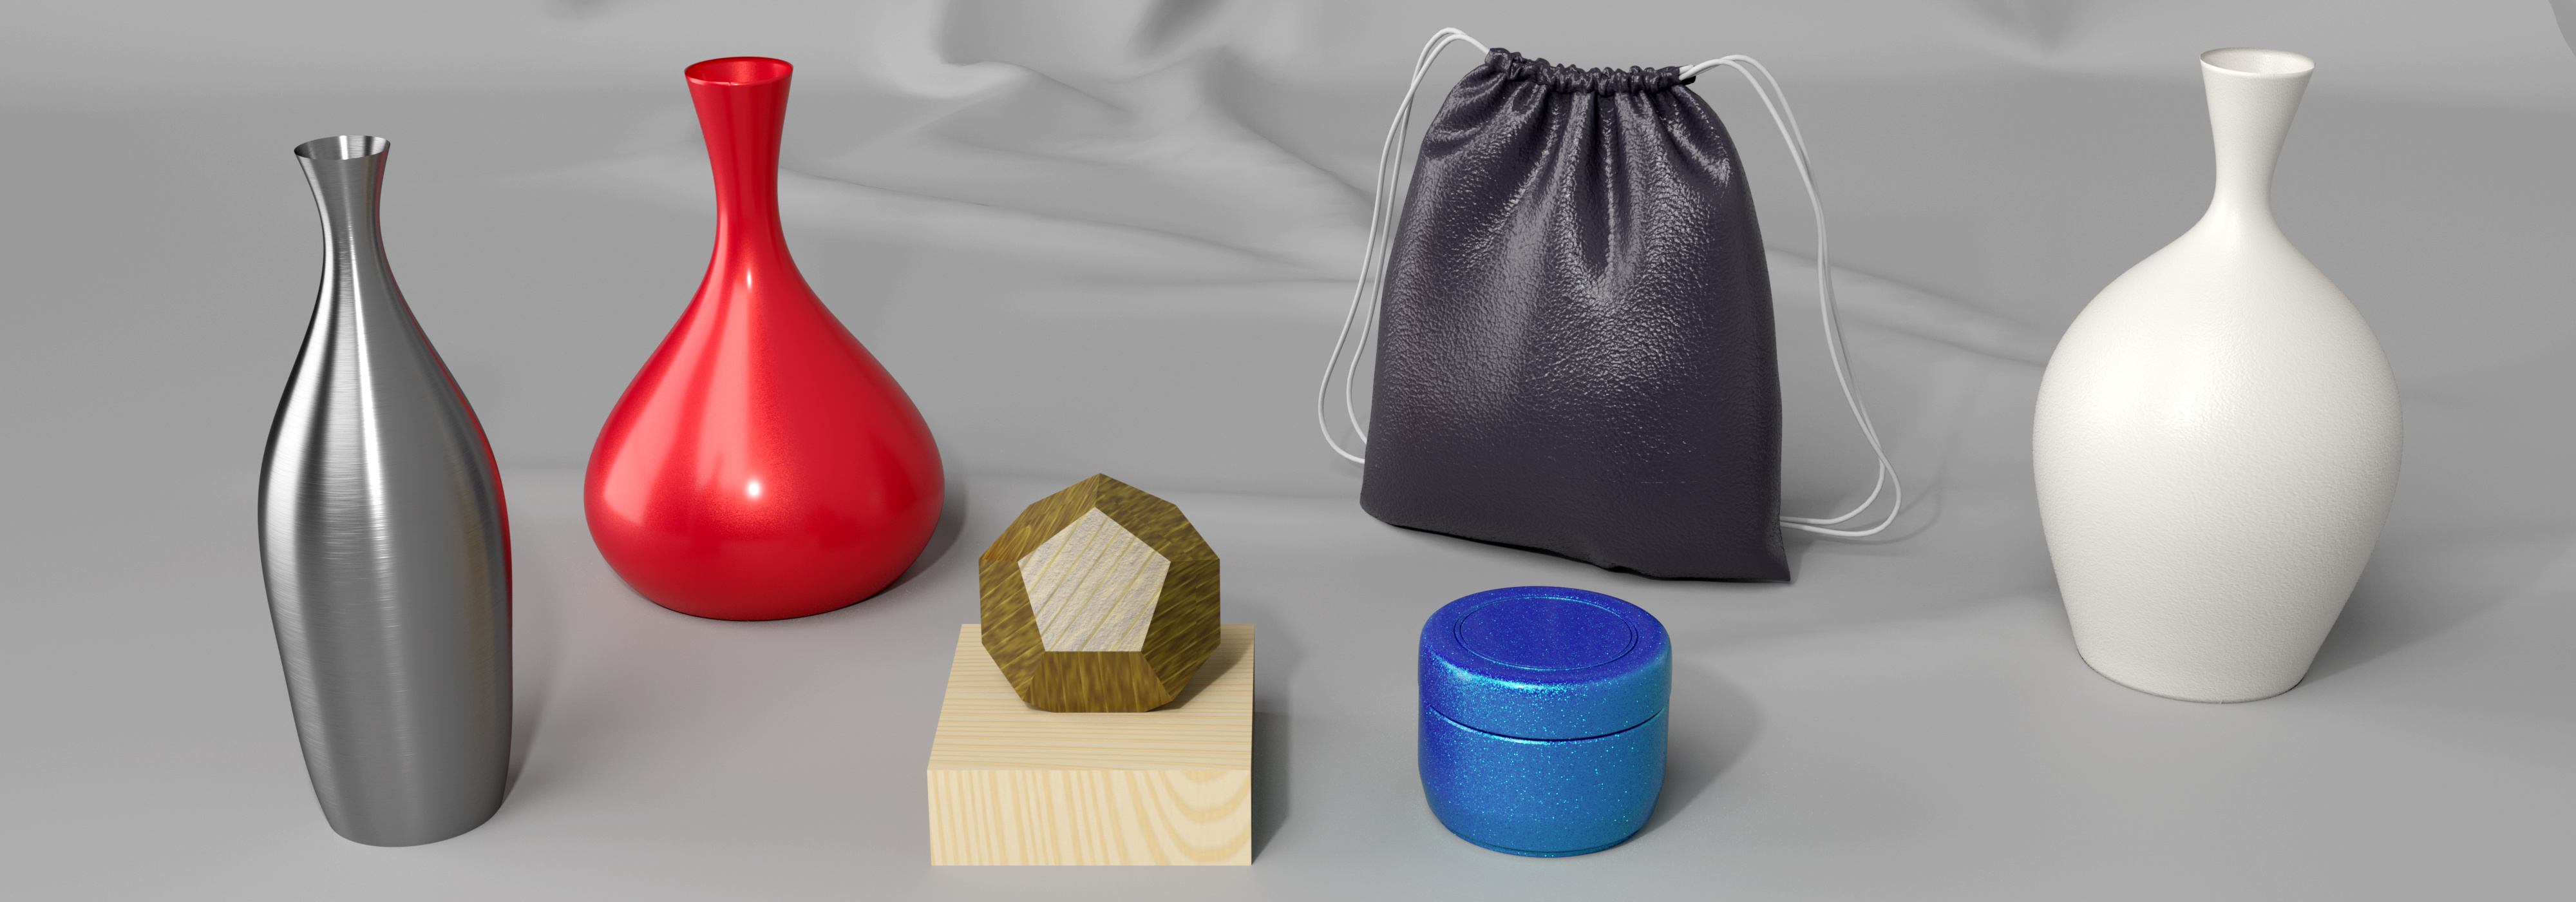
\includegraphics[width=\textwidth]{images/img/teaser.png}\\[3pt]
	\iftrue
		\setlength{\insetLen}{0.134\textwidth}
		\begin{tabular}{cccccccc}
			\raisebox{3pt}{\rotatebox{90}{\small \bfseries Rendered}} &
			\adjincludegraphics[width=\insetLen,trim={0 {.2\height} 0 {.2\height}},clip]{images/real/metal/out/good1.png} &
			\adjincludegraphics[width=\insetLen,trim={0 {.2\height} 0 {.2\height}},clip]{images/real/flake2/out/good1.png} &
			\adjincludegraphics[width=\insetLen,trim={0 {.2\height} 0 {.2\height}},clip]{images/real/wood2/out/good1.png} &
			\adjincludegraphics[width=\insetLen,trim={0 {.2\height} 0 {.2\height}},clip]{images/real/wood3/out/good1.png} &
			\adjincludegraphics[width=\insetLen,trim={0 {.2\height} 0 {.2\height}},clip]{images/synth/flake/out/good1.jpg} &
			\adjincludegraphics[width=\insetLen,trim={0 {.2\height} 0 {.2\height}},clip]{images/real/leather/out/good1.jpg} &
			\adjincludegraphics[width=\insetLen,trim={0 {.2\height} 0 {.2\height}},clip]{images/real/bump2/out/good1.png}
			\\
			\raisebox{7pt}{\rotatebox{90}{\small \bfseries Target}} &
			\adjincludegraphics[width=\insetLen,trim={0 {.2\height} 0 {.2\height}},clip]{images/real/metal/out/target.png} &
			\adjincludegraphics[width=\insetLen,trim={0 {.2\height} 0 {.2\height}},clip]{images/real/flake2/out/target.png} &
			\adjincludegraphics[width=\insetLen,trim={0 {.2\height} 0 {.2\height}},clip]{images/real/wood2/out/target.png} &
			\adjincludegraphics[width=\insetLen,trim={0 {.2\height} 0 {.2\height}},clip]{images/real/wood3/out/target.png} &
			\adjincludegraphics[width=\insetLen,trim={0 {.2\height} 0 {.2\height}},clip]{images/synth/flake/out/target.jpg} &
			\adjincludegraphics[width=\insetLen,trim={0 {.2\height} 0 {.2\height}},clip]{images/real/leather/out/target.jpg} &
			\adjincludegraphics[width=\insetLen,trim={0 {.2\height} 0 {.2\height}},clip]{images/real/bump2/out/target.png}
		\end{tabular}
	\else
		\setlength{\insetLen}{0.137\textwidth}
		\begin{tabular}{ccccccc}
			\begin{overpic}[width=\insetLen]{images/img/teaser_metal1.png}
				\imglabel{Brushmetal-3}
			\end{overpic}
			&
			\begin{overpic}[width=\insetLen]{images/img/teaser_flake1.png}
				\imglabel{Metallicflake-3}
			\end{overpic}
			&
			\begin{overpic}[width=\insetLen]{images/img/teaser_wood2.png}
				\imglabel{Wood-4}
			\end{overpic}
			&
			\begin{overpic}[width=\insetLen]{images/img/teaser_wood1.png}
				\imglabel{Wood-3}
			\end{overpic}
			&
			\begin{overpic}[width=\insetLen]{images/img/teaser_flake2.png}
				\imglabel{Metallicflake-1}
			\end{overpic}
			&
			\begin{overpic}[width=\insetLen]{images/img/teaser_leather1.png}
				\imglabel{Leather-3}
			\end{overpic}
			&
			\begin{overpic}[width=\insetLen]{images/img/teaser_bump2.png}
				\imglabel{Bump-4}
			\end{overpic}
		\end{tabular}
	\fi
	\caption{
			A scene rendered with material parameters estimated using our method: bumpy dielectrics, leather, plaster, wood, brushed metal, and metallic paint. The insets show a few examples of the input (target) images, and renderings produced using our procedural models with parameters found by Bayesian posterior sampling.
		\vspace{3mm}
 	}
	\label{fig:teaser}
}
